%!TEX root = ../main.tex
\chapter{绪论}
\label{chap:intro}

现代大型直线加速器应用,如 X 射线自由电子激光 XFEL、直线正负电子对撞机、超快电子衍射 UED、汤姆逊散射源 TSS 等对电子束品质提出了很高的要求。下面以 XFEL,MeV UED 和 TSS 为例,简要介绍各应用对束流品质的需求。

\section{现代直线加速器应用对低发射度束流的需求}
描述电子束品质常用的参数有发射度、峰值流强、亮度等;其中发射度描述了束团在相空间中所占体积大小,可分为横向发射度和纵向发射度。横向发射度越小,一般意味着束团的横向尺寸与准直性越好;纵向发射度越小,一般意味着束团的纵向长度与能散越小。
\subsection{XFEL}
描述 XFEL 的几个重要公式如下\cite{Huang:2007aa}:
\begin{eqnarray}
\rho &=& \left[\frac{1}{16}\frac{I_e}{I_A}\frac{K_0^2[JJ]^2}{\gamma_0^3\sigma_x^2k_u^2}\right]^{1/3}\\
P_{\text{sat}} &=& \rho P_e\\
L^{\text{1D}}_{G} &=& \frac{\lambda_u}{4\pi\sqrt{3}\rho}\\
\frac{\varepsilon_n}{\gamma_0} &\le& \frac{\lambda}{4\pi}\\
\sigma_{\eta} &\ll& \rho
\end{eqnarray}
其中 $\rho$ 为皮尔斯参数,它决定了 XFEL 饱和功率 $P_{\text{sat}}$ 、增益长度 $L^{\text{1D}}_{G}$(正比于出光功率饱和所需的波荡器长度)以及所能容忍的束团能散;$\rho$ 越大,饱和功率越大,增益长度越小,所能容忍的束团能散就越大,XFEL 表现就越好。可以看出 $\rho$ 与束团尺寸 $\sigma_x$ 成反比,因此要求束团尺寸越小越好。对于 XFEL 的 X 射线,其波长越短,要求发射度 $\varepsilon_n$ 越小,因此 XFEL 要求束团有尽可能小的横向尺寸以及发射度。图 \ref{fig:xfel} 针对 PSI 的 SwissFEL\cite{Patterson:2010aa},给出了 XFEL 出光功率随束团发射度的关系,可以看出,若能将束流发射度从 \emit{0.4} 降至 \emit{0.1},XFEL 出光功率可以提高一个量级。
\begin{figure}[htbp]
\centering
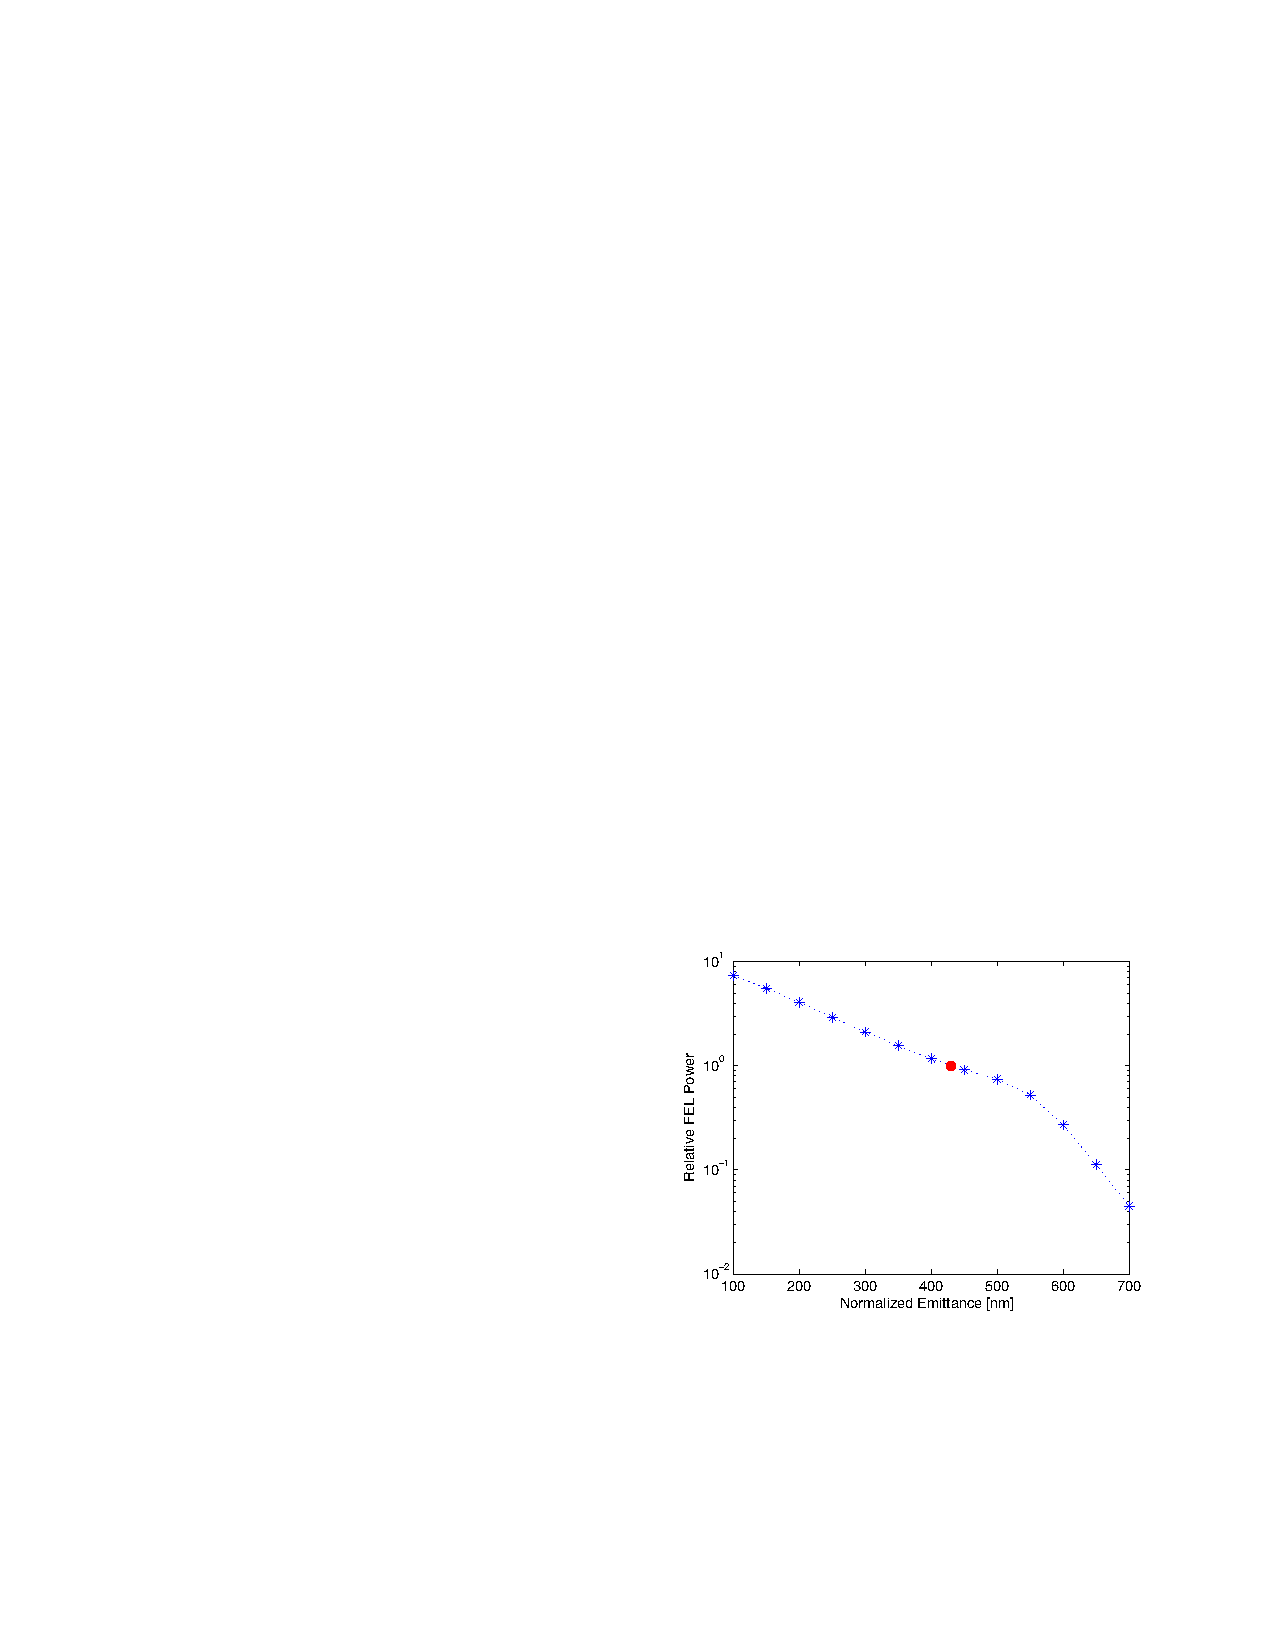
\includegraphics[width=0.6\textwidth]{xfel}
\caption{\label{fig:xfel} FEL 功率随发射度的变化\cite{prat2014emittance}。}
\end{figure}

\subsection{MeV UED 对束流品质的需求}
MeV UED 即兆电子伏超快电子衍射,是一种将超短的 MeV 电子束作为探针,观察物质结构的实验手段。其原理见图 \ref{fig:ued}。
\begin{figure}[htbp]
\centering
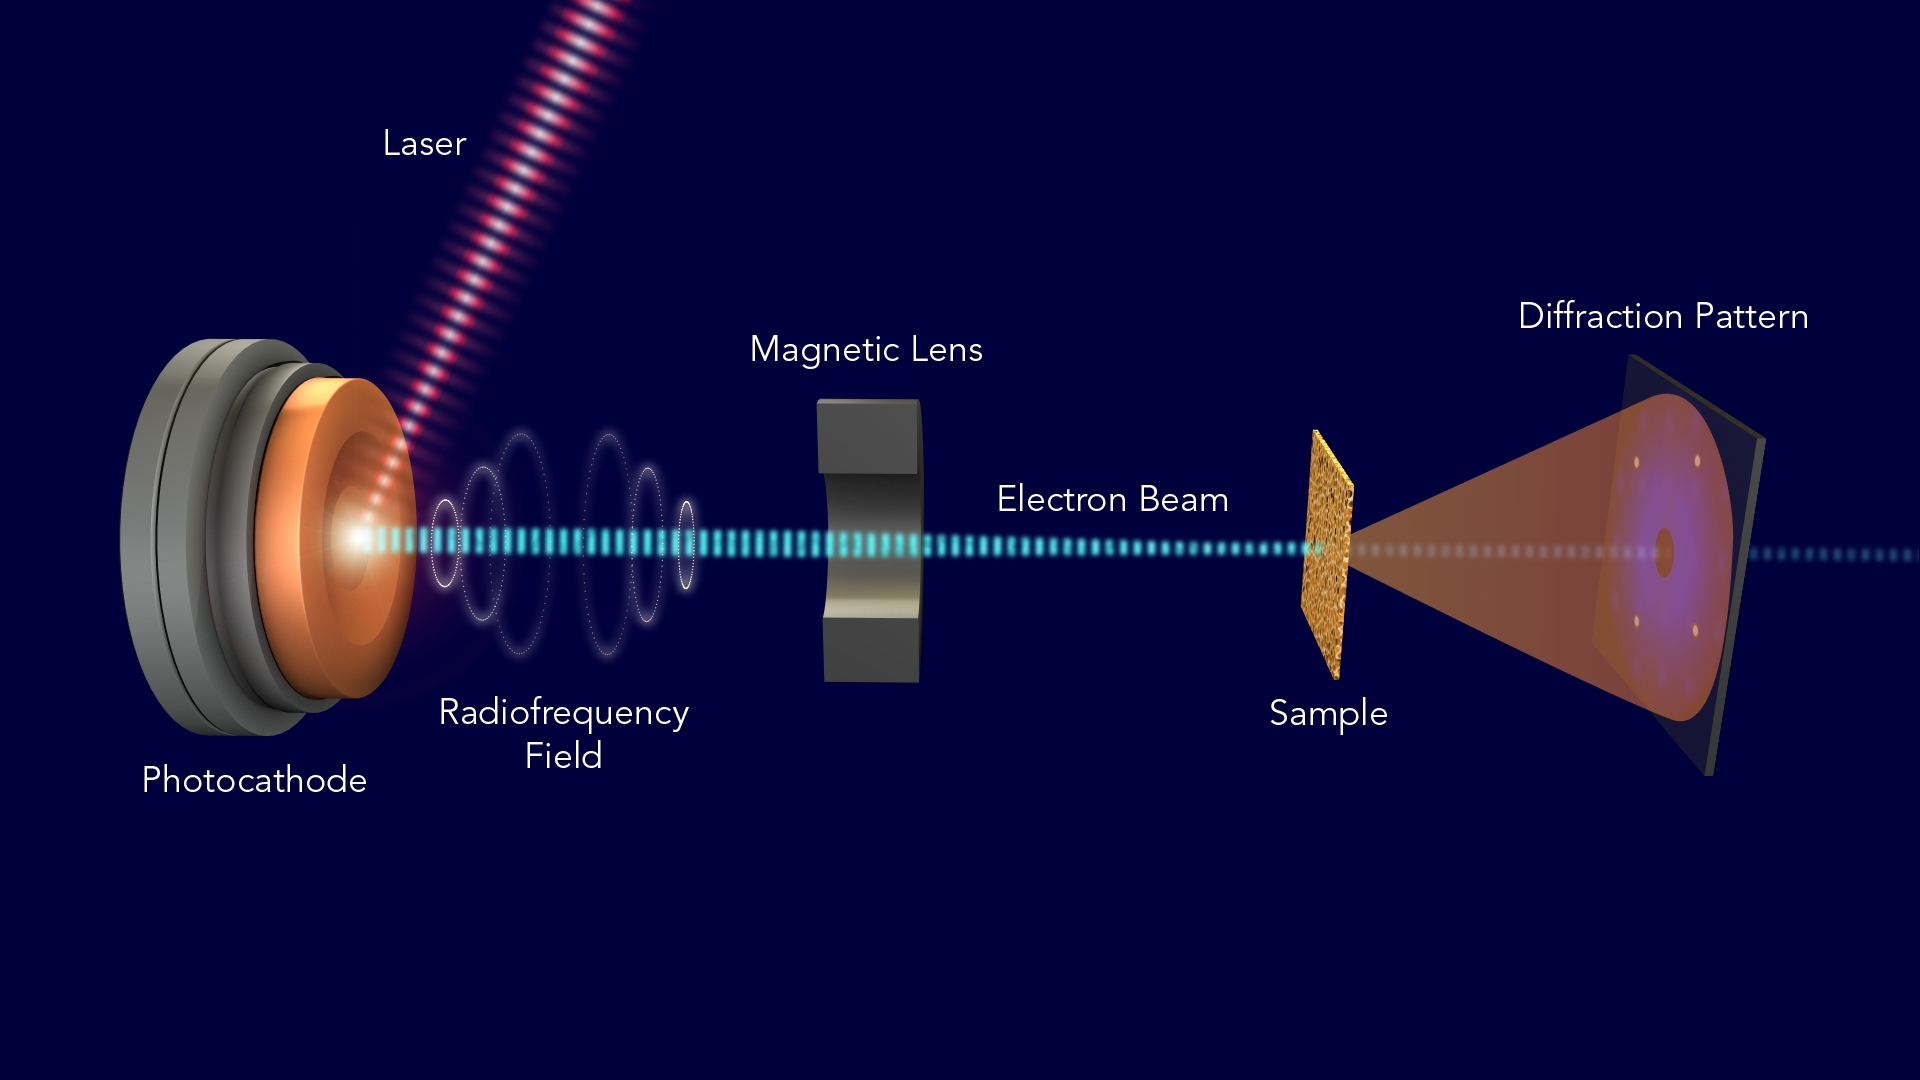
\includegraphics[width=0.8\textwidth]{ued}
\caption{\label{fig:ued} MeV UED 原理图\cite{Li:aa}。}
\end{figure}

MeV UED 的空间和时间分辨率如下式描述\cite{Weathersby:2015aa}:
\begin{eqnarray}
\Delta s &=& \frac{2\pi}{\lambda_e}\frac{\varepsilon_n}{\sigma_x}\\
\tau &=& \sqrt{\tau_e^2+\tau_{\text{ph}}^2+\tau_{\text{TOA}}^2+\tau_{\text{VM}}^2}
\end{eqnarray}
其中 $\lambda_e$ 为电子的康普顿波长。由上式可见在电子探针横向尺寸 $\sigma_x$(样品上的电子束团 rms 尺寸)一定的情况下,空间分辨率随发射度 $\varepsilon_{n}$ 降低而降低,也即能分辨更细微的结构。同时电子的纵向尺寸越小,其时间分辨率也越小。一般 MeV UED 为保证足够的时间和空间分辨率,工作在低电荷量模式,电荷量 $Q < \SI{1}{pC}$,要求发射度 $\varepsilon_{n} < \SI{0.1}{mm\cdot mrad}$(达到 $<\SI{0.01}{mm\cdot mrad}$ 更好),束长尽量短($<\SI{1}{ps}$,若能达到 fs 量级更好)。根据发射度对电荷量的放缩关系($\varepsilon_n\propto\sqrt{Q}$),可知其发射度相当于 200\,pC 时 \emit{1.4}(达到更理想分辨率则需要 \emit{0.14}),其难度可见一斑。

\subsection{汤姆逊散射源对束流品质的需求}
汤姆逊散射源通过光子与较高能电子对撞,产生背向散射的高能 X 射线\cite{Milburn:1963aa,Fiocco:1963aa}。汤姆逊散射源的原理见图 \ref{fig:ttx}。
\begin{figure}[htbp]
\centering
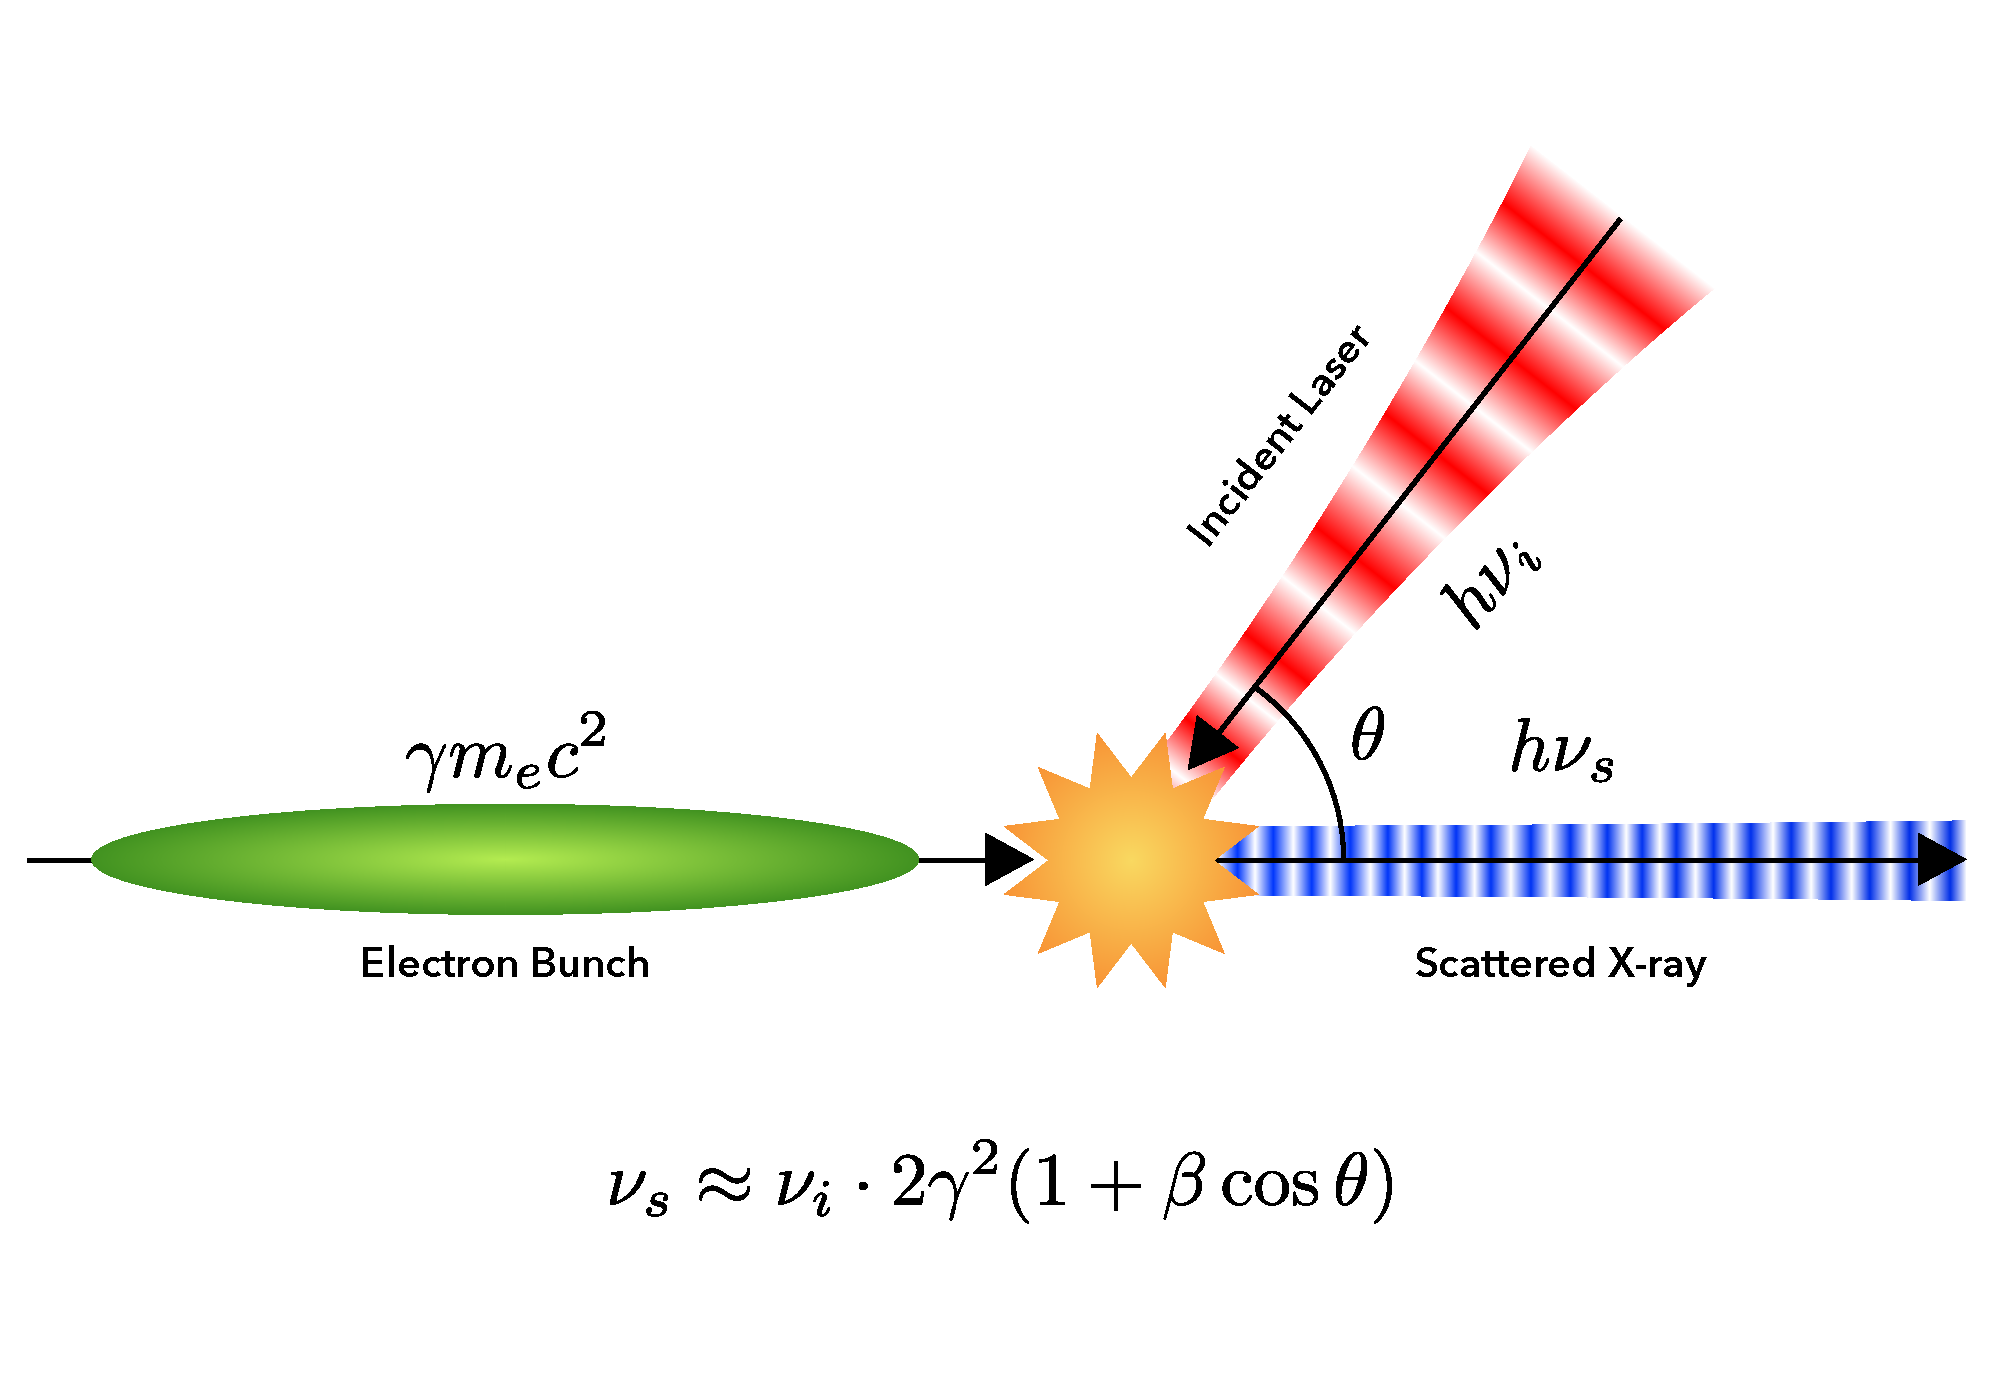
\includegraphics[width=0.6\textwidth]{ttx}
\caption{\label{fig:ttx} MeV UED 原理图。}
\end{figure}

激光与电子束正面对撞时,X 射线产额最大,此时 X 射线光子总数 $n_x$ 满足\cite{huangwenhui:2004aa}:
\begin{equation}
n_x = C_{\text{off}}\frac{n_en_l}{2\pi}\Sigma_{\text{th}}\frac{1}{\sqrt{(\sigma_{ex}^2+\sigma_{lx}^2)(\sigma_{ey}^2+\sigma_{ly}^2)}}
\end{equation}
其中 $n_e, \sigma_{ex}, \sigma_{ey}$ 是电子束的电子数目,x 向和 y 向尺寸;$n_l, \sigma_{lx}, \sigma_{ly}$ 是激光束的光子数目,x 向和 y 向尺寸。当电子束能散可忽略时,汤姆逊散射 X 射线源的亮度 $B_x$ 满足\cite{duyingchao:2006aa}:
\begin{equation}
B_x \propto \frac{n_x}{\varepsilon_{n, x}^2\varepsilon_{n, y}^2}
\end{equation}
从以上两式可知,电子束团发射度越小,X 射线光子总数越大,X 射线源亮度越高。对于清华大学加速器实验室的汤姆逊 X 射线散射源,需求电荷量 1\,nC,发射度 \emit{1} 以下的电子束团\cite{Qian:2012aa}。

\section{光阴极,光阴极微波电子枪与光阴极注入器}
为提供低发射度束流,常常采用光阴极注入器。光阴极注入器由光阴极微波电子枪,发射度补偿螺线管线圈和四极铁等束流操控元件及若干段加速管组成,其中光阴极微波电子枪是其核心。光阴极微波电子枪利用光电效应在光阴极表面产生电子束团,随后利用腔体内的高梯度射频场(几十至上百 MV/m),快速将束流加速到较高能量(几个到十几个 MeV),以抑制束团低能阶段空间电荷力对束流品质的破坏。

光阴极微波电子枪通过激光控制电子束团发射,可以产生超短束团,其阴极电流密度很大,因此适用于产生亮度很高的电子束团。在电子束团产生后,需要对电子束团进行进一步加速,并在加速过程中保持电子束的高亮度,这就是光阴极注入器的意义。

\section{基于光阴极注入器的低发射度束流发展现状}
如上节所述,激光入射光阴极微波电子枪的光阴极,通过光电效应激发光电子产生,光电子随后在电子枪中的高梯度射频场中加速,经过螺线管线圈,四极磁铁等束流操控元件以及加速管进行进一步能量提升,最终抵达注入器出口。束流在光阴极表面产生时的发射度叫做热发射度,它决定了注入器出口处的束流发射度的最小值;然而,注入器出口束流发射度一般要大于热发射度,这是因为电子束在注入器的整个运动过程中,有很多因素都会造成发射度增长。追踪一个束流从产生到出射注入器的全部过程,就可更清晰地看到这些因素的影响。从光阴极表面出射时,由于阴极的粗糙度,可能造成热发射度的增长;激光入射粗糙表面时可能会激起表面等离激元,也会对发射度有一定影响。在电子枪的射频场运动时,线性和非线性 RF 效应都会造成投影发射度增长。在螺线管线圈中,尽管发射度得到了补偿,但色散效应又会增大发射度。

自二十世纪八十年代起,经过二十多年的努力,人们已经逐步消除或补偿了其中的几个因素造成的发射度增长,下面简单回顾一下基于光阴极注入器的低发射度束流的发展。

\begin{figure}[htbp]
\centering
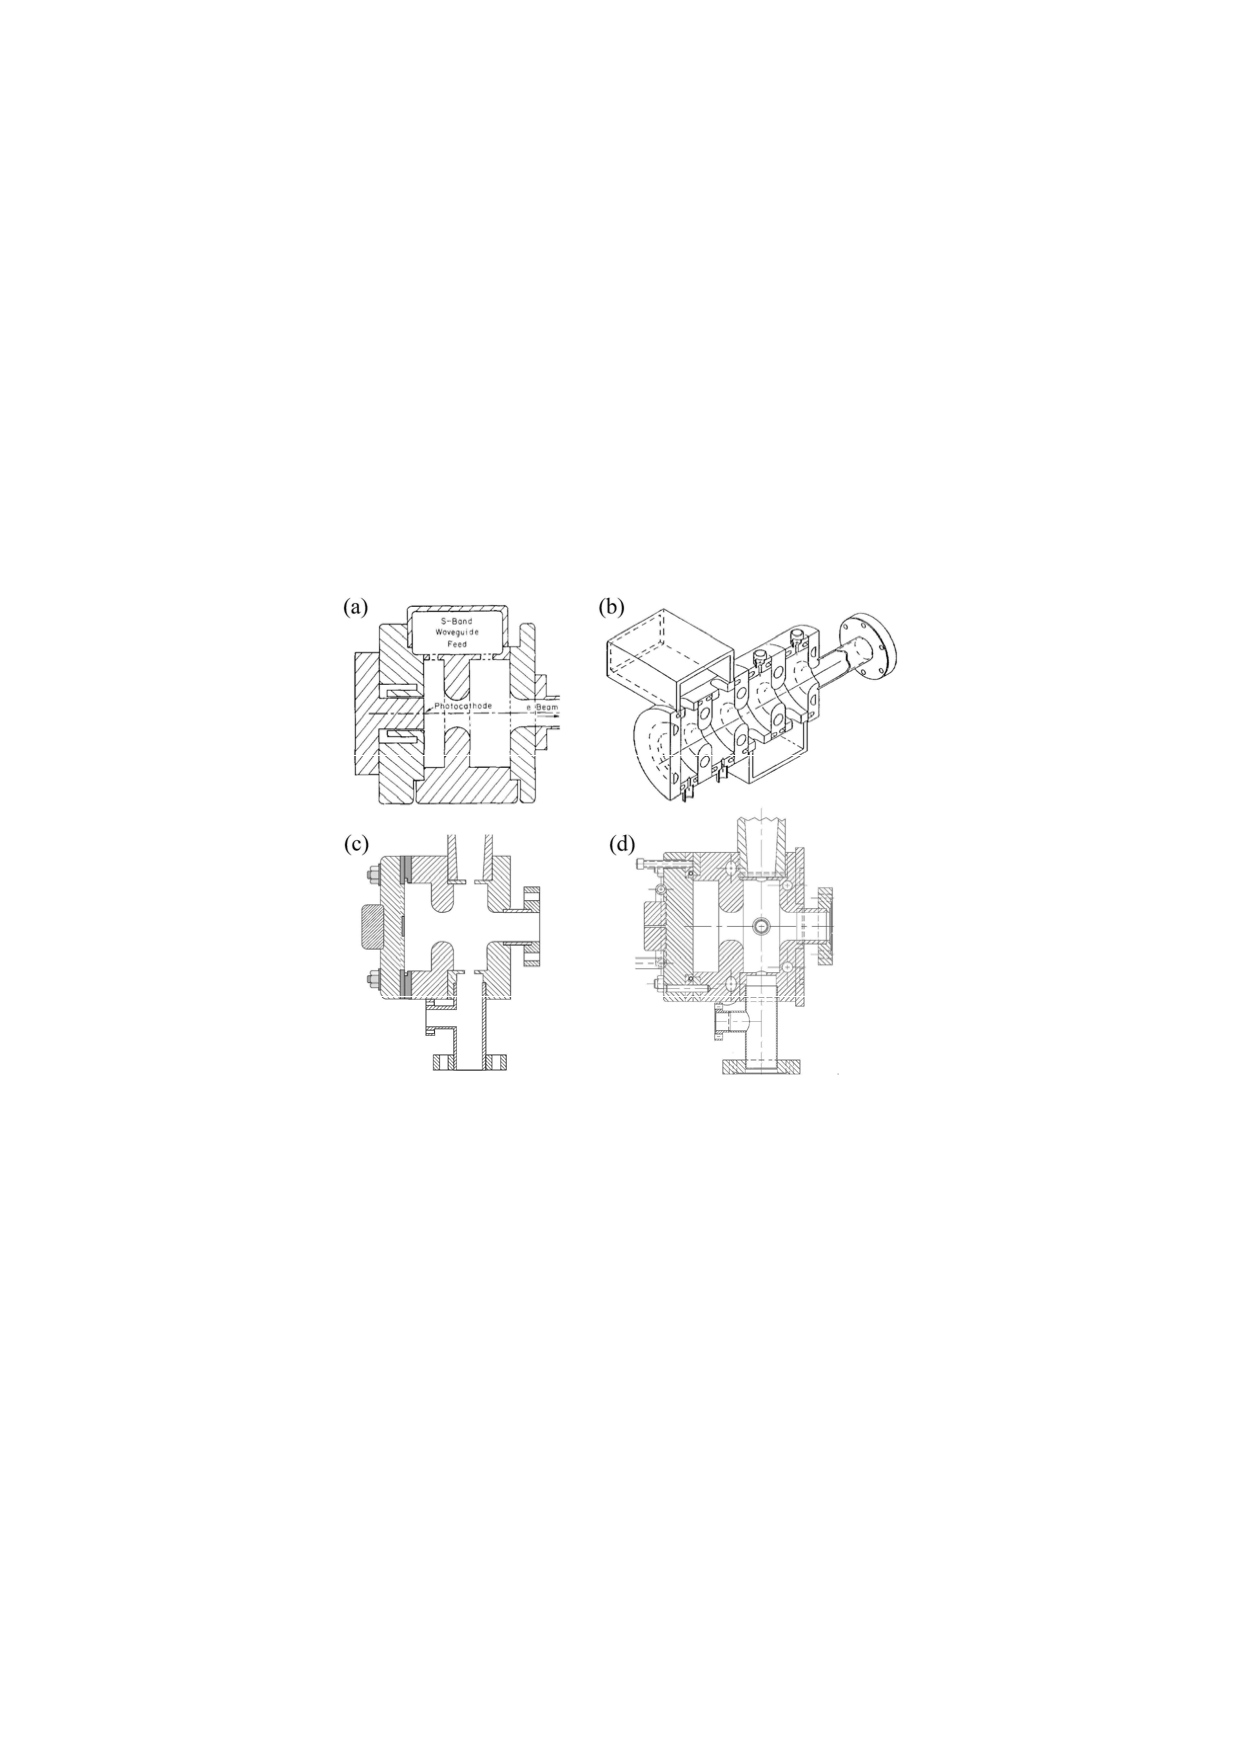
\includegraphics[width=0.7\textwidth]{guns}
\caption{\label{fig:guns} S 波段光阴极微波电子枪结构示意图\cite{Qian:2012aa}。}
\end{figure}

第一阶段在 1985 年光阴极微波电子枪注入器搭建成功\cite{Fraser:1986aa,Fraser:1987aa}后开始。该阶段光阴极注入器出口处发射度主要由电子枪本身限制,因此优化主要集中在抑制电子枪中线性/非线性 RF 场及空间电荷力造成的切片和投影发射度增长。McDonald 给出了电子枪理想边界,使横向 RF 场为线性\cite{McDonald:1988aa};Kim 解析了光阴极微波电子枪中束流的运动,并提出通过减小束团纵横比来抑制空间电荷力发射度增长,以及减小束团长度来抑制纵向非线性 RF 发射度增长\cite{Kim:1989ab};为进一步抑制非线性空间电荷力,增大阴极表面场强从而有首腔 0.5 cell 的设计\cite{McDonald:1988aa};同时为补偿关联投影发射度提出在电子枪上应用螺线管线圈\cite{Carlsten:1989aa}。

第二阶段则在上一阶段基础上,进一步优化电子枪结构,以消除多极场/干扰模式对发射度的影响,进一步提高束团亮度。为达到对束团更强聚焦以及束长压缩以提高束团亮度,首腔从 0.5 cell 变到 0.6 cell\cite{Lehrman:1992aa};由于关联发射度增长被抑制,电子枪中多极场对发射度的改变显现出来,因此电子枪结构/功率馈入变得对称化\cite{Palmer:1998aa},并采用跑道型耦合孔抑制多极模\cite{Limborg:2005vn, Akre:2008aa};$\pi$ 模工作时激发起的 0 模对发射度造成影响,因此优化束流孔以扩大频率间隔\cite{Palmer:1998aa}。电子枪腔型的发展过程见图 \ref{fig:guns}。

第三阶段中,电子枪的腔型造成的发射度增长已经很小,注入器出口处的发射度近似由热发射度、非线性 RF 发射度及非线性空间电荷发射度组成\cite{Qiu:1996aa}。此阶段人们开始优化整个注入器结构及激光参数。针对非线性空间电荷力,KV 分布\cite{Kapchinskij:1959aa}被动力学模拟证明可以有效抑制非线性空间电荷力发射度增长\cite{Limborg-Deprey:2006aa,Khojoyan:2013aa},进而激光整形、扁平束发射(pancake regime)\cite{bazarov2009maximum}及笔形束发射(cigar regime)\cite{filippetto2014maximum}等可以产生 KV 分布束团的方法被提出及模拟或实验验证\cite{Khojoyan:2013aa,Khojoyan:2014aa,Musumeci:2008ab,Li:2012aa}。对于非线性 RF 作用,Dowell 和 Raguin 分别提出了两种空间叠合型双频电子枪\cite{Dowell:2004aa,Raguin:2005aa}以实现纵向线性 RF 场,消除非线性 RF 发射度增长。

第四阶段,也即当前阶段中,注入器出口处的发射度已迫近热发射度\cite{li2012multi,gulliford2013demonstration,karkare2011effect,},此时阴极的地位变得重要:阴极材料的选取\cite{Cultrera:2014ab},阴极表面形态(表面粗糙度,污染)\cite{Vecchione:2012aa,Vecchione:2013aa,Ling:2013aa},以及阴极表面上的物理过程:肖特基效应,空间电荷限等都会对注入器出口处发射度产生较大影响\cite{qian2012experimental}。在这个阶段中,人们提出了光阴极表面极限亮度并进行了实验验证\cite{bazarov2009maximum,filippetto2014maximum}。

综合以上,对注入器出口束流品质的优化基本分为两个部分,即对光阴极表面热发射度的优化,以及对注入器多个参数的优化,以将光阴极的横向亮度保持到注入器出口。下面详细介绍这两部分的相关研究和进展。

\subsection{光阴极热发射度的优化}
\subsubsection{改变材料及激光波长}
对于光阴极上的热发射度,Dowell 采用三步模型给出了金属光阴极体发射情形的发射度\cite{Dowell:2006aa,dowell2009quantum}:
\[
	\varepsilon_{n} =\sigma\sqrt{\dfrac{\hbar\omega-\phi_{\mathrm{eff}}}{3mc^2}}
\]
该公式揭示了体发射情形热发射度与金属材料及激光波长的关系。该公式催生了一系列调变金属材料与激光波长来优化热发射度的研究,如 PSI 对四种不同金属阴极热发射度及量子效率的实验\cite{hauri2010intrinsic},实验中使用了可微调中心波长的激光,通过对每种金属扫描激光波长,同步测量发射度与 QE 变化来验证理论公式。实验中测量了四种金属阴极:Cu,Mo,Nb,Al。实验直接验证了可以通过减小光子能量与有效逸出功的差距来降低热发射度,也同时验证了热发射度降低时,其对应的 QE 也会降低。该实验的结论是 Cu 是最适合用来做光阴极的金属。当入射光光子能波长为 282 nm,引出场强为 25 MV/m  时,Cu 的归一化热发射度为 0.41\,mm$\cdot$mrad/mm,QE 为 $5\times10^{-6}$。

\subsubsection{采用新的发射机制}
人们提出了光场使能的场致发射(Photo Field Emission,PFE)来从原理上降低热发射度\cite{Reifenberger:1979aa}。光场使能场致发射本质上是一种场致发射,场致发射是利用量子隧穿效应的电子发射机制,其好处在于出射电子横向动量极小,因此可以有很低发射度,缺点是依靠高梯度微波场发射时其发射束团长度较长(ns 量级)且电荷量较小。若用激光作用于场致发射阴极(一般是针尖或针尖阵列)上,可以提高电子能量,使隧穿概率升高,本不能场致发射的场强下也可进行场致发射。PFE 结合了场致发射发射度低和光电发射可控以及可产生超短束团的优点。PFE 提出后,针对 XFEL 上的应用陆续有实验\cite{Ganter:2008aa,Mingels:2012aa,Mingels:2013aa,Mingels:2014aa}及模拟研究\cite{Fallahi:2014aa}开展。如采用单 ZrC 针尖(半径 5\,$\mu$m)阴极,阴阳极之间加 60\,kV,2\,ns,30\,Hz 的脉冲高压,使用 16\,ps,266\,nm 的短束长激光入射就可以获得高 QE(针尖附近场强高)的同时实现低发射度。PFE 发射理论上可以在引出电荷 150\,pC 时获得 \emit{0.05} 的发射度。

\subsubsection{抑制阴极表面效应}
金属阴极表面一般有表面污染及表面粗糙起伏,这也会造成发射度的变化。表面污染一般是阴极加工时引入,例如电抛光时引入的 S、C、O 等元素。实验研究证明不同污染主要影响金属表面逸出功\cite{Chelvayohan:1982aa,Opower:2006aa,Valizadeh:2013aa}。例如对于银阴极,表面的硫污染会导致逸出功升高,表面的碳污染却会导致逸出功降低\cite{Chelvayohan:1982aa}。应对阴极表面污染造成的硬性,目前较常见的解决方法是激光清洗\cite{Brachmann:2011aa}以及 Ar 原子轰击清洁阴极表面\cite{Chelvayohan:1982aa,Valizadeh:2013aa}。实验证明,利用 Ar 原子清洁可使阴极表面的 C 和 O 含量大幅降低,对量子效率的提升有很大帮助\cite{Valizadeh:2013aa};利用激光清洗,减小激光功率,缩短激光扫描步长,也会对量子效率有显著提升\cite{Brachmann:2011aa}。

另外对于光阴极微波电子枪中常用的多晶铜(晶面可能为(100),(110) 和 (111))阴极,研究发现阴极表面晶面不同的位置其逸出功也不同,且可能有高达 400\,meV 的差别\cite{Renault:2006aa},这也会引起热发射度的增长。可能的解决方案是采用单晶铜阴极,受限于单晶金属的造价,一般采用 cathode-plug 的方式进行应用\cite{Ganter:2013aa}。

对于阴极表面粗糙度造成的热发射度增长的研究,一般采用二维正弦表面模型进行研究\cite{He:2004aa,Krasilnikov:2006aa,Karkare:2011aa}。阴极表面粗糙度热发射度增长主要来自两方面:即表面离散效应(slope effect)和横向电场效应(field effect)\cite{Bradley:1977aa}。阴极的粗糙度被认为是造成热发射度实验测量值与理论值差异的主要原因\cite{qian2012experimental,Vecchione:2012aa,schubert2013bi}。尽管有基于二维正弦表面的定性粗糙度热发射度公式对两种增长效应给出物理上的解释,但是由于缺乏针对一般粗糙阴极表面的粗糙度热发射度公式(slope effect 主要是数学上的困难,field effect 主要是物理上的困难),粗糙度热发射度公式中的参数主要靠实验拟合,其说服力有限,且目前无法给出想抑制粗糙度热发射度到一个水平以下,对表面加工的要求具体是多少。

阴极表面粗糙度在合适激光波长的作用下有可能激励起表面等离激元\cite{Novotny:2012aa}。表面等离激元的产生对光阴极亮度既有好处又有坏处:表面等离激元可以将光子囚禁在金属阴极表面,这会增大阴极对激光的吸收率,同时表面等离激元会极大加强阴极上的激光功率密度,进而提高 QE;但另一方面,表面等离激元所要求的粗糙阴极表面形态会造成发射度的增长,这会降低阴极亮度。利用表面等离激元性质的阴极有两类:衰减全反射阴极(ATR)和纳米表面阴极(NPC)。其中衰减全反射阴极利用棱镜在金属薄膜表面激发表面等离激元,既有高 QE 的优点又兼具平面阴极低发射度的优点,但其问题在于由于微波的趋肤深度一般大于金属薄膜厚度,会造成场泄漏,难以集成在光阴极微波电子枪中\cite{Watanabe:2011aa,Neo:2012aa};而 NPC 阴极经实验验证,当工作在多光子光电发射模式\cite{Musumeci:2010aa},其电子产额有上百倍的增长,且归一化热发射度相对于平整阴极只增长不到 1 倍\cite{Polyakov:2013ab,Li:2013ac},因此是有潜力产生高亮度束团的候选。目前对于 NPC 阴极的研究仅限于铜阴极(材料易获得易加工),其他材料的发射特性有待研究。

\subsection{光阴极注入器中发射度的保持}
热发射度的优化和光阴极注入器的优化是密不可分的:即使在阴极表面产生了超低热发射度,因其可能存在的非线性空间电荷力和非线性 RF 场作用,也极有可能无法将超低热发射度保持到光阴极出口。因此进行光阴极注入器优化时,需要同时考虑阴极上的激光参数。下面介绍光阴极注入器优化的重要进展和工作。

\subsubsection{最高场强的优化}
提高电子枪及加速管的工作频率可以提高腔内最大场强,可更有效地抑制束流发射阶段空间电荷力发射度增长。目前世界范围内绝大多数注入器均采用 S 波段或 L 波段(LCLS 采用 L 波段注入器\cite{Zhou:2015aa},PSI 采用 S 波段注入器\cite{prat2014emittance},Cornell 注入器束线中也是 S 波段加速管\cite{Bartnik:2015aa},DESY 的 PITZ 注入器中采用 L 波段电子枪\cite{Krasilnikov:2012aa})Limborg 于 2011 年搭建了 X 波段光阴极注入器测量平台\cite{Limborg-Deprey:2011aa},第一台 X 波段光阴极注入器于 2016 年成功搭建\cite{Limborg-Deprey:2016aa},其中阴极发射场强高达 150\,MV/m,其 100\,pC 对应发射度为 \emit{0.7},虽然发射度较大但其纵向 rms 束长极短,只有 400\,fs,亮度很高。另外一个提高注入器最高场强的办法是降低阴极温度\cite{Rosenzweig:2016aa}。研究发现,当电子枪运行于低温($\sim$ 20\,K)时,其表面所允许的最大场强大幅上升,可以利用这个性质来进一步抑制束团发射阶段的非线性空间电荷效应。

\subsubsection{自动优化算法}
由于光阴极优化的多输入变量多优化目标的本质(优化发射度时要同时兼顾峰值流强),多目标进化算法最早于 2005 年被 Bazarov 应用于光阴极注入器优化\cite{Bazarov:2005aa}。在该工作中,Bazarov 将 NSGA-II 遗传算法\cite{Deb:2002aa} 应用于 Cornell 的直流高压枪注入器优化,遗传算法优化器对于 100\,pC 情形给出了 \emit{0.1} 的结果,对于 1\,nC 情形给出了 \emit{0.7} 的结果,从而证明了遗传算法优化器的可靠性与相对于人工的优势,即可能获得全局最优解。Qiang 将差异进化算法(differential evolution algorithm)应用于类 LCLS 的注入器优化,由于算法的贪婪本质,大大缩短了遗传算法优化所需要的时间\cite{Qiang:2013aa},当然与此同时带来的问题是可能无法获得全局最优解。Bettoni 受遗传算法启发,将分段单纯形法应用于 SwissFEL 注入器束线优化中,并获得 10\,pC 电荷量下 \emit{0.08} 以及 200\,pC 电荷量下 \emit{0.14} 的优化结果\cite{Bettoni:2015aa}。

\subsubsection{激光参数的优化}
KV 分布\cite{Kapchinskij:1959aa}可以有效抑制非线性空间电荷力发射度增长\cite{Limborg-Deprey:2006aa,Khojoyan:2013aa},相对于常用的柱形均匀分布束团,三维均匀椭球束团的注入器出口处发射度可降低 30\%\cite{Khojoyan:2014aa}。产生 KV 分布的束团目前常用的有三种方法:激光整形、扁平束发射(pancake regime)及笔形束发射(cigar regime),其对发射度增长的抑制效果已被实验初步验证\cite{Khojoyan:2013aa,Khojoyan:2014aa,Musumeci:2008ab,Li:2012aa}。目前激光整形技术精度不够,离三维均匀椭球尚有一定偏差,这会造成不小的发射度增长\cite{Khojoyan:2013aa};扁平束在发射过程中,由于其极强的纵向空间电荷力,扁平束流会在很短时间内纵向膨胀成为一个准 KV 分布束团,但由于阴极表面的镜像电荷效应,初始服从 KV 分布的束团若电荷量太大会出现畸变,因此只限于产生低流强的束团\cite{Musumeci:2008ab};笔形束与扁平束正相反,靠其极强的横向空间电荷力,在发射后迅速横向膨胀成为一个准 KV 分布束团,且由于其横向尺寸很小,可产生 nm 级发射度\cite{Li:2012aa}。最近的遗传算法优化发现,将阴极上的初始束长拉长,有助于保持阴极热发射度,在注入器出口处可获得更低发射度的束流\cite{Qian:2016aa}。

\subsection{低束流发射度的测量}
优化获得注入器出口处的低发射度束流后,还需进行实验测量已验证优化效果,下面介绍低发射度束流的常用发射度测量方法。根据束流发射度的统计定义,束流发射度由横向束斑尺寸与横向动量参数共同决定。实验中,电子束的横向束斑尺寸信息可通过荧光屏上的束流图像直接测得~\cite{Graves:1997aa,Walasek-Hohne:2011aa},因此,发射度的测量问题主要集中在对束流的横向动量信息的获取~\cite{lee2015review}。

为叙述方便起见,引入平均横向动能(Mean Transverse Energy,MTE)的概念\cite{bazarov2008thermal,bazarov2009maximum,lee2015review}:
\begin{equation}
\text{MTE} = \frac{1}{2}m\langle v_\perp^2\rangle
\end{equation}
其中 $m$是电子质量,$v_\perp$为电子的横向速度。MTE与光阴极束流归一化热发射度 $\Delta_{x}$ 关系如下:
\begin{equation}
\label{eq:es_MTE}
\Delta_{x} = \sqrt{\frac{\text{MTE}}{mc^2}}
\end{equation}

目前,已有多项研究对MTE的数值进行理论推导~\cite{karkare2011effect,karkare2013monte}与实验测量~\cite{bazarov2009maximum,engelen2014effective,dowell2009quantum,qian2012experimental}。但是对于超低发射度的测量依然处以探索研究阶段,下面主要介绍针对 $\text{MTE}<\SI{100}{meV}$(等效归一化热发射度 $<$ 0.4\,mm$\cdot$mrad/mm)的发射度测量~\cite{hauri2010intrinsic,lee2015review}。

\begin{table}[htbp]
\caption{常用的发射度测量方法}
\label{tab:method}
\centering
\begin{tabular}{p{2cm}p{3.5cm}p{5cm}p{2.5cm}}
\toprule
方法 & 测量设置 & 方法的不足 & MTE测量值 \\
\midrule
半球形分析仪~\cite{Palczewski:2010aa} & 施加不同的电压来区分测量不同能量、不同空间分布的发射电子 &1)对功函数敏感;2)非直接的测量;3)易被系统中的杂散电磁场干扰;4)当发射电子动能小于1\,eV时测量结果不可靠;5)不适用于强场(MV/m)电子枪环境 & $\sim$ 100\,meV~\cite{Droubay:2014aa} \\
渡越时间分析器~\cite{Wang:2012aa,Sertore:2004aa}  & 利用延迟线探测器测量发射电子的渡越时间和横向位置 &1)需要一个亚皮秒的激光;2)易被环境中的电磁场干扰;3)当发射电子动能小于1\,eV时测量结果不可靠;4)不适用于强场(MV/m)电子枪环境 & $\sim$130$\pm$5\,meV~\cite{sertore2004cesium} \\
能量分析谱仪~\cite{Karkare:2015aa,Orlov:2001aa} & 测量发射电子在纵向磁场下的运动 & 1)不适用于强场(MV/m)电子枪环境;2)纵向磁场也许会影响光电发射的过程,测量结果不准 & $\sim$25$\pm$2.5\,meV~\cite{Orlov:2001aa} \\
最小束斑扫描法~\cite{engelen2014effective,bazarov2008thermal,bazarov2011thermal,anderson2002space,hauri2010intrinsic} & 电子枪加聚焦元件组 & 需要准确的磁场标定测量 &  $\sim$1\,meV~\cite{engelen2014effective}\\
束流采样或胡椒瓶法~\cite{anderson2002space,Reiser:2008aa,gulliford2013demonstration} & 两片光栅加探测器或者一片光栅加探测器 & 对于低MTE的束流,分辨率与束流初始发射度相当 & 35\,meV ~\cite{Maxson:2015aa}\\
自由膨胀法~\cite{feng2015novel} & 加速结构和自由漂移段 & 1)存在激光衍射效应;2)需要极小的激光光斑;3)使用的网格不均匀 & 27\,meV~\cite{feng2015novel} \\
横向能散谱仪~\cite{jones2013commissioning}  & 在加速段中自由膨胀 & 1)需要极小的激光光斑; 2)无法应用在kV/m的环境中 & $\sim$45$\pm$7\,meV~\cite{jones2013commissioning} \\
\bottomrule
\end{tabular}
\end{table}

对于目前有的发射度测量方式,其总结与对比可参见表格 \ref{tab:method}\cite{lee2015review}。其中典型的几个方法简介如下:

(1)半球形分析器\cite{Palczewski:2010aa}和渡越时间探测器\cite{Wang:2012aa, Sertore:2004aa}常用于角分辨的光电子能谱(Angle Resolved Photoemission Spectroscopy,ARPES)测量实验中~\cite{Palczewski:2010aa,Zhang:2011aa}。采用能量大于材料逸出功的光子照射在材料表面,利用半球形分析器或者渡越时间探测器测量发射电子的能量、对应的方位、极化角分布等参数,通过对测量材料的旋转,可以获得全角度范围的光电子信息,从而统计给出MTE参数。由于低能的发射电子(<1\,eV)易受系统中杂散电磁场的干扰,该系统适用于发射电子能量在几个eV能量范围~\cite{Droubay:2014aa,Sertore:2004aa}。

(2)最小束斑扫描法常用于加速器光阴极注入器的在线发射度测量~\cite{engelen2014effective,bazarov2008thermal,bazarov2011thermal,anderson2002space,hauri2010intrinsic},根据聚焦元件的种类,也称为螺线管扫描法或者四极磁铁扫描法。其装置设置的简单示意图如图~\ref{fig:waist_scan}(a)所示,电子经过电场的加速后,进入漂移段,通过改变磁透镜(螺线管或四极磁铁)的电流,改变其对束流的聚焦焦距,从而改变束流的包络。采用荧光屏和相机观测记录一定距离之后的束斑尺寸,束斑尺寸大小随着透镜强度的变化如图~\ref{fig:waist_scan}(b)中所示的曲线。根据束流传输理论,当所有传输元件(加速段、聚焦元件等)为线性元件,线性传输矩阵记为$\bf{\text{R}}=\bf{\text{R}}_{i\to f}$,描述束流从位置$i$到位置$f$的束斑联系矩阵,即~\cite{bazarov2008thermal}:
\begin{equation}
\label{eq:waist_scan}
\left(\sigma_x \sigma_{\theta_x}\right)_f = R\left(\sigma_x \sigma_{\theta_x}\right)_i
\end{equation}
其中,束流参数包含了rms束斑尺寸$\sigma_x$和rms束流发散角$\sigma_{\theta_x}$。由于$\bf{\text{R}}$已知,多组测量拟合下,可反推获得束流初始,即光阴极出口处的发射度(或者MTE)的信息。该方案需要对传输矩阵以及荧光屏上的束斑尺寸进行准确测量,传输元件的非线性效应、非线性空间电荷力效应等会引起测量误差、同时,该方案对于超低发射度的测量需要提高相机、荧光屏对束斑尺寸的分辨率。
\begin{figure}[htbp]
\centering
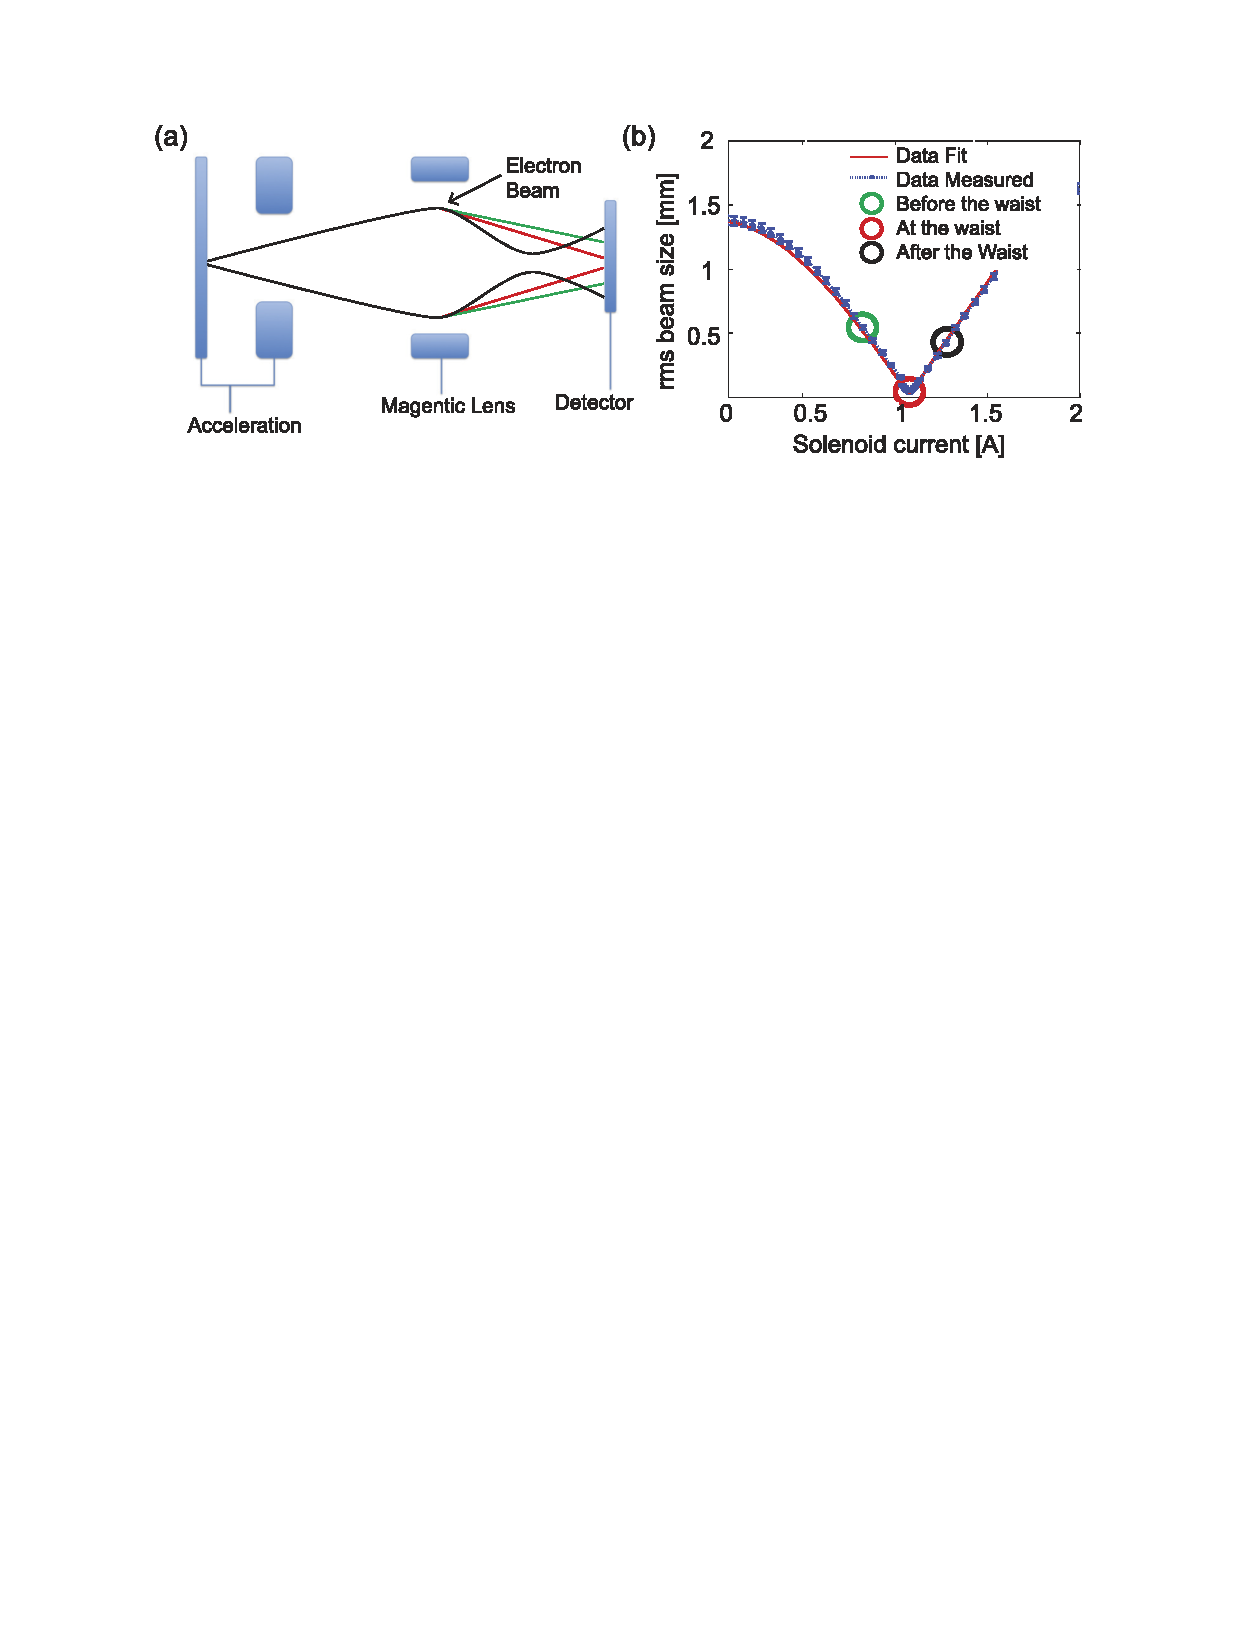
\includegraphics[width=0.9\textwidth]{waist_scan}
\caption{\label{fig:waist_scan} 最小束斑扫描法原理示意图}
\end{figure}

(3)束流采样或者胡椒瓶盖法\cite{anderson2002space,gulliford2013demonstration,li2012nanometer}:这类方法的主要优点是可以扫描获取整个束流的横向相空间。在两个窄缝系统的束流采样方案中,两个带有窄缝金属平板相隔一定距离,放置于束流前进方向,由于平板足够厚,只有窄缝位置处的束流可以通过。第一个窄缝选择出距离束斑中心一定位置的一定范围内的部分电子,被选择出来的电子进一步漂移,通过第二个窄缝的筛选,只有几个电子被最终的探测器(如测量电荷量的法拉第桶)收集,通过扫描窄缝的位置,该方法可以获取整个束流的横向分布与横向散角分布,从而获得束流的横向相空间。胡椒瓶法是对上述方案的改良,用胡椒瓶盖形状的栅网对束流进行采样,采用偏转腔替代法拉第筒对筛选后的束流进行偏转测量,可同时测量切片相空间。但是该类方法的分辨率受限于窄缝金属板厚度与之间的间隔,分辨率与MTE数值相当,同时,电子束与窄缝平板或胡椒瓶盖栅网的散射等作用对测量也可能造成误差影响~\cite{Reiser:2008aa,Maxson:2015aa}。

(4)自由膨胀法或者横向动量谱仪~\cite{feng2015novel,jones2013commissioning},都是简单地使得发射电子在空间自由运动开,通过测量一定距离后的横向束斑尺寸,来反推初始的MTE参数。如图 \ref{fig:free_expand} 所示,采用一束聚焦到极小光斑(rms尺寸<100\,$\mu$ m)的激光入射,产生初始的电子束,经历阴极和阳极之间的高梯度加速场后,漂移至探测屏测量其横向束斑尺寸。整个系统中,阳极是一个精细的电子显微镜栅网设计,阳极栅网结构足够小,以至于阳极网格的散焦力影响可忽略,阳极与阴极之间的电场只在电子轨迹方向对束流进行加速,因此可以较为精确地测量MTE的数值\cite{jones2013commissioning}。
\begin{figure}[htbp]
\centering
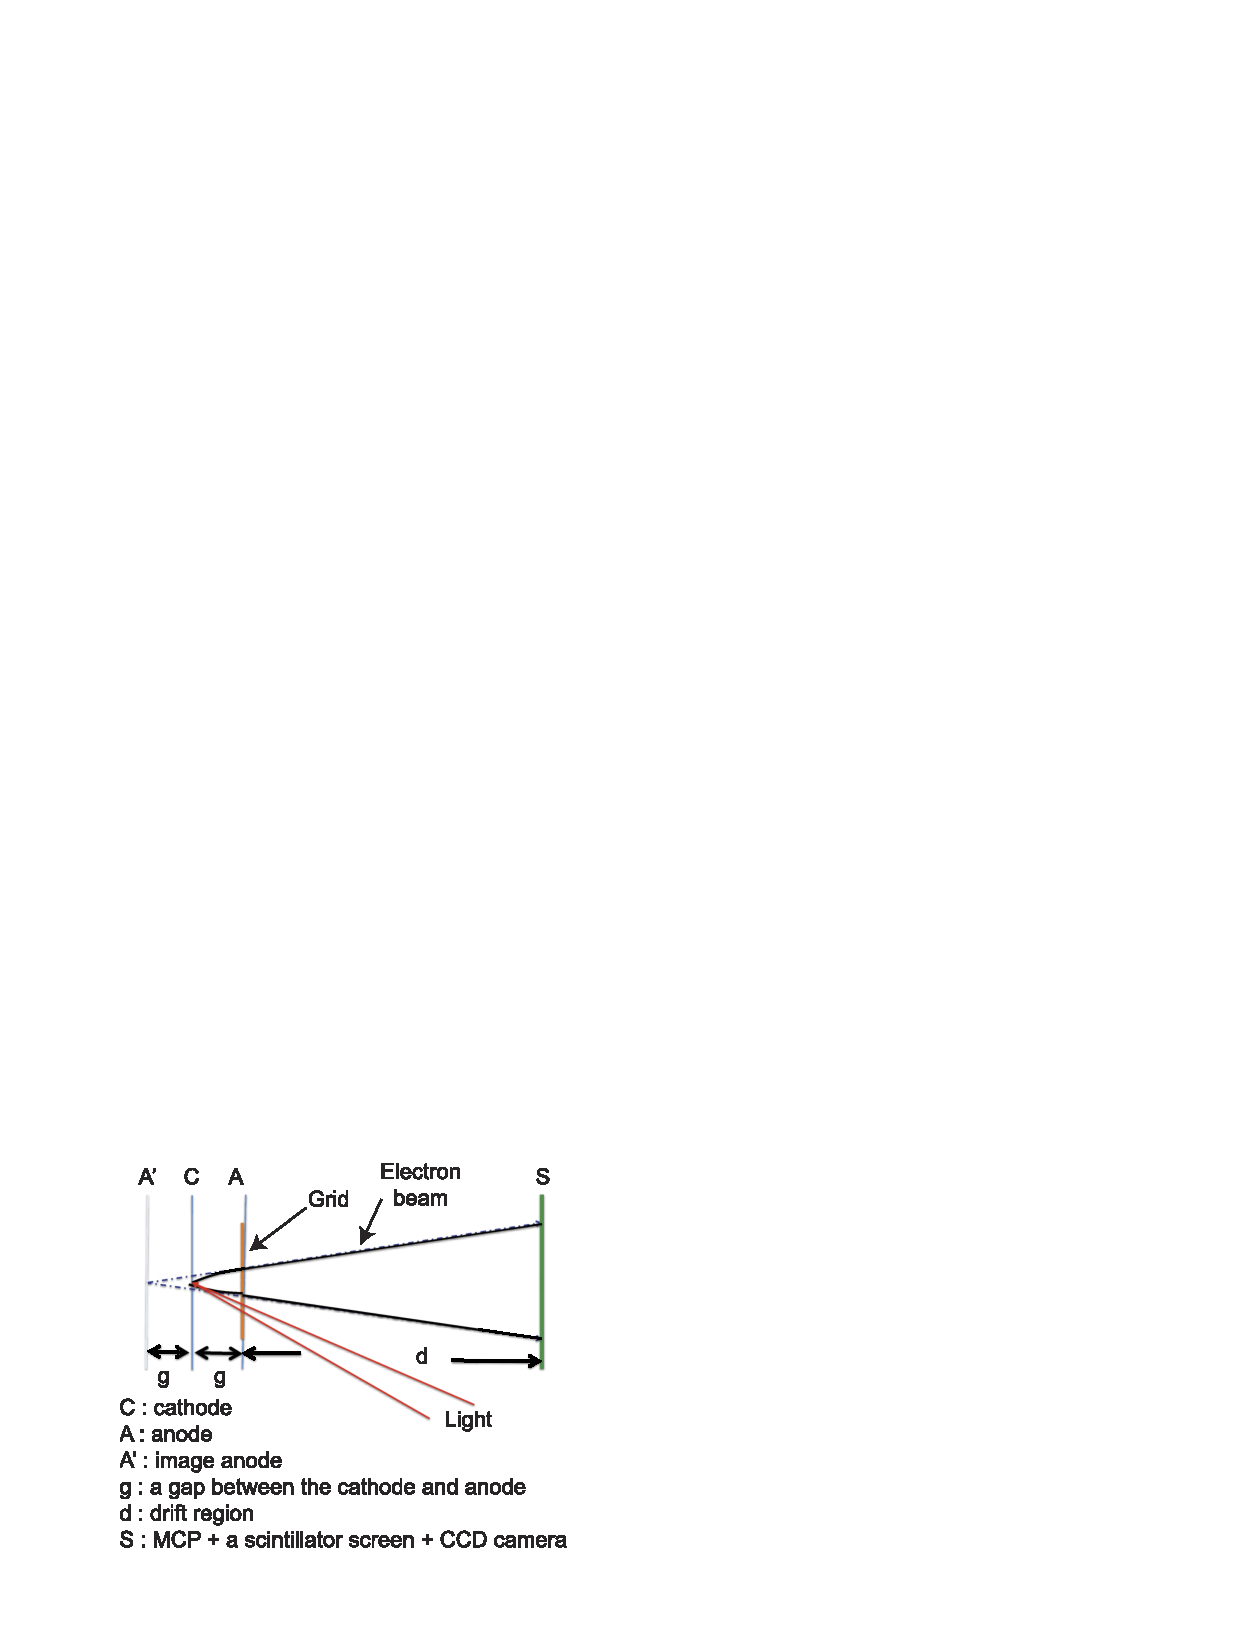
\includegraphics[width=0.6\textwidth]{free_expand}
\caption{\label{fig:free_expand} 自由膨胀法测量MTE的原理示意图}
\end{figure}

几个重要加速器应用的光阴极注入器出口束流参数最新测量值见表 \ref{tab:record-emit}。
\begin{table}[htbp]
\caption{几个重要装置注入器出口束流参数的实验测量结果}
\label{tab:record-emit}
\centering
\begin{tabular}{lcccccl}
\toprule
波段 & 峰值场强 & 发射场强 & 枪电压 & 发射度 & 峰值流强 & 装置 \\
 & MV/m & MV/m & MV & $\mu$m & A & \\
\midrule
S-band & $\sim$ 100 & $\sim$ 50 & $\sim$ 5 & $\sim$ 0.2--0.45 & 20--50 & LCLS/PSI \\
L-band & $\sim$ 60 & $\sim$ 45 & $\sim$ 7 & $\sim$ 0.3 & 15 & PITZ \\
DC & $\sim$ 4 & $\sim$ 4 & $\sim$ 0.4 & $\sim$ 0.6 & 30 & Cornell \\
VHF & $\sim$ 20 & $\sim$ 20 & $\sim$ 0.8 & $\sim$ 0.45 & 30 & APEX \\
\bottomrule
\end{tabular}
\end{table}

\section{论文工作的主要内容与创新点}
通过多年发展,光阴极出口处的束流发射度逐渐逼近热发射度,目前实验测量最优的结果是 200\,pC 电荷量下 \emit{0.2} 切片发射度及 \emit{0.3} 投影发射度。200\,pC 束团的发射度是否已达到极限?我们的课题围绕这一问题进行探索,并尝试给出答案。如前所述,光阴极出口处束流发射度决定于初始束流热发射度,以及后续传输过程中对发射度的保持。束流在阴极表面产生时,阴极表面粗糙度对其贡献大小会影响后续的电子枪及注入器优化(抑制空间电荷效应发射度增长要尽量增大表面电场,但若表面粗糙度的横向电场发射度太大则增大表面电场会使热发射度增大,得不偿失),因此定量研究清楚一般阴极表面上粗糙度热发射度贡献大小对发射度优化有重要的意义;阴极上另一效应表面等离激元对束团亮度的影响不定,目前虽已有针对铜表面等离激元阴极的研究,但其它材料的发射属性依然未知,是否有新材料能够超越铜纳米阴极的亮度是一个值得探究的问题;阴极上的极限亮度已有公式给出,对于能够有效保持初始发射度到注入器尾端的扁平束和笔形束而言,若能从理论上预言其热发射度的极限,会对光阴极出口处发射度的优化有重要的参考意义;注入器的遗传算法优化表明要拉长初始束团可以抑制非线性空间电荷发射度增长,以降低注入器出口处发射度,但初始长度过长又会引入纵向非线性 RF 发射度,若能设法将非线性 RF 发射度补偿,就可能在注入器出口处获得更低(200\,pC 下 $\sim$ \emit{0.1})的发射度。论文工作主要围绕着以上几个问题逐步展开。

\subsection{论文工作的主要内容}
本论文主要内容如下:

(1)将点扩散函数的概念引入光阴极热发射度计算中,应用点扩散函数的观点给出了一般随机缓变粗糙表面阴极的表面离散效应和横向电场效应造成的粗糙度热发射度解析公式,并对一块真实阴极上光电发射过程中束团相空间及粗糙度热发射度的演化进行了数值模拟。模拟得到的真实阴极上的粗糙度热发射度与解析公式给出的符合较好。通过解析公式及数值模拟,发现对于三维随机缓变粗糙表面及粗糙度参数与其匹配的二维缓变粗糙表面,表面粗糙度对于发射度增长的贡献明显低于预期值。在阴极表面场强高达 120\,MV/m 时,发射度增长因子也低于 1.1,与发射度测量的一系列实验的测量值 1.5 $\sim$ 2 有较大差距。对于一块经过精细打磨的阴极(表面 rms 起伏不超过 \SI{30}{nm},表面 rms 坡度不大于 \SI{3}{mrad}),在阴极表面电场不太高($\sim$ 50\,MV/m)时表面粗糙度造成的发射度增长可以忽略不计。详细内容见第三章。

(2)模拟及实验探究了银纳米表面阴极的发射特性。先采用宽带反射率谱仪对表面刻有纳米结构的银晶片进行反射率谱测量,再将银晶片放入电子枪中进行高功率测试。银纳米表面晶片 266\,nm 激光下的量子效率 QE 测量值是 2.2$\times10^{-5}$,800\,nm 激光下的电子产额增益约为 400,x 向和 y 向的归一化热发射度分别为 1.6\,mm$\cdot$mrad/mm 和 1.7\,mm$\cdot$mrad/mm。多光子光电发射测量表明相同激光功率密度下,银纳米阴极相较于铜纳米阴极可以产生更高的电荷密度,但同时热发射度也要比铜纳米阴极大约 15\%。与平滑铜阴极相比,热发射度高了近一倍。我们也讨论了实验中观察到的一些有趣现象,如高功率测试后银纳米结构的损坏,离线反射率谱测量中 600\,nm 处奇怪的谐振峰,电子枪中由于 cathode-plug 设计造成的一系列效应等等。详细内容见第四章。

(3)理论计算了光阴极表面扁平束发射和笔形束发射两种情形下的极限热发射度,从极限热发射度的角度说明笔形束相对于扁平束的优势;针对笔形束发射中的非线性力导致的发射度增长问题,提出了分离型双频光阴极微波电子枪的概念,并用遗传算法对包含空间分离双频电子枪的注入器束线进行了多变量多目标优化。优化结果表明,在普通电子枪后引入一个高频腔可以将注入器出口处 \SI{200}{pC},峰值流强 \SI{30}{A} 的束流的发射度降低 $\sim$ 25\%,且切片发射度近乎与热发射度相等,这意味着双频电子枪成功将束流的初始横向亮度保持到注入器出口。当归一化热发射度降低至 \SI{0.5}{\mu m/mm} 时,优化器给出了注入器出口处流强 \SI{30}{A} 时切片发射度 $\sim$ \emit{0.10} 的方案。详细内容见第五章。

\subsection{论文工作的主要创新点}
本论文创新点如下:

(1)通过将点扩散函数引入光阴极热发射度计算,首次解析计算并数值模拟了真实粗糙表面阴极的粗糙度热发射度增长。理论及模拟结果表明,对于一块经过精细打磨的阴极(表面 rms 起伏不超过 \SI{30}{nm},表面 rms 坡度不大于 \SI{3}{mrad}),在阴极表面电场不太高($\sim$ 50\,MV/m)时表面粗糙度造成的发射度增长可以忽略不计。

(2)首次对银材料的纳米表面阴极发射属性进行了系统的高功率测量。实验结果表明银纳米阴极相较于铜纳米阴极可以产生更高的电荷密度,但同时热发射度也要比铜纳米阴极更大,因此适用于需要高电荷量且对发射度要求不太高的场景。

(3)首次理论上给出了扁平束发射和笔形束发射的极限热发射度,提出了采用分离型双频光阴极微波电子枪抑制非线性力发射度增长的方案,并用遗传算法进行了动力学优化验证。优化结果表明高频腔的引入可将光阴极的热发射度保持到注入器出口,并给出了注入器出口处流强 \SI{30}{A},切片发射度 $\sim$ \emit{0.10} 的方案。
